
\graphicspath{{Chapter2/Figs/}}

\setcounter{chapter}{5}
\chapter*{Capítulo 2} 
\addcontentsline{toc}{chapter}{Capítulo 2}
\setcounter{figure}{0}
\setcounter{table}{0}
\setcounter{section}{0}

{\LARGE Estudios genómicos sobre la biogénesis de precursores de miARNs en plantas}

\section{Introducción}
En nuestro grupo se está estudiando la biogénesis de miARNs, específicamente como los precursores son reconocidos y procesados en plantas \citep{Bologna2013}.
Ya que la misma depende del reconocimiento de claves estructurales ubicadas en los precursores de miARN \citep{pmid21554756,citeulike:8816489,Bologna11112012}.
Estos precursores tienen una estructura de tallo-burbuja característica \citep{Jones-Rhoades2006}, que se cree que proporciona las claves para el procesamiento del mismo y la liberación de los ARN pequeños de 21 nt.

Los precursores de miARNs en plantas son muy variables en tamaño y forma \citep{Bologna2013,citeulike:8816489}.
Esa variabilidad se puede observar entre distintas familias de precursores, pero a veces también entre una misma familia de precursores en distintas especies (Figura \ref{fig:hairpin_distribution}).

\begin{figure}[htbp!] 
    \centering    
    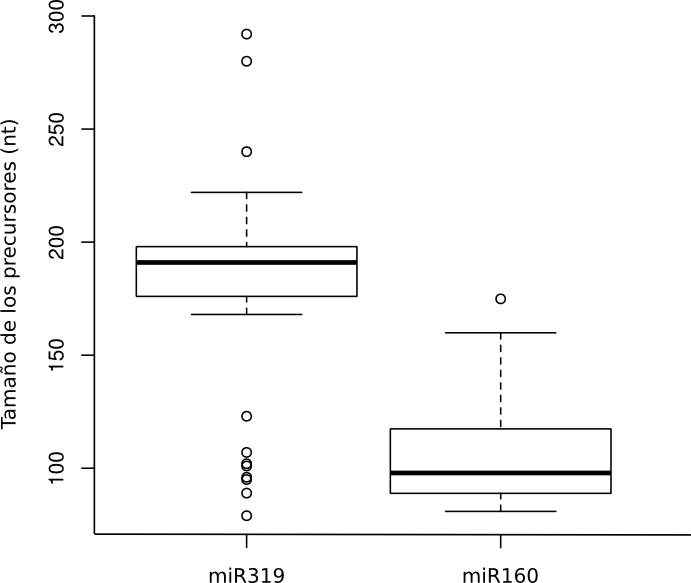
\includegraphics[width=.6\textwidth]{hairpin_distribution.png}
    \caption[Tamaño de precursores]{Tamaño de precursores. Se muestra el tamaño (nt) de dos familias de precursores en distintas especies.}
    \label{fig:hairpin_distribution}
\end{figure}

Además, en las plantas, las mutaciones que impiden la biogénesis o actividad de los miARNs, tales como \textit{hyl1}, \textit{hen1} y \textit{ago1}, conducen al aumento en los niveles de los transcriptos de muchos de los genes blanco de miARNs (aproximadamente un 45\% de todos los blancos) \citep{Han2004,pmid12747833,pmid16889646,Allen2005207}.
Esto sugiere que el mecanismo que involucra el corte y degradación de los ARNm es un componente importante de la represión inducida por los miARNs en plantas \citep{Jones-Rhoades2006, Voinnet2009669}.

En particular, la biogénesis de los miARNs es un proceso clave porque determina la secuencia exacta de nucleótidos del ARN pequeño funcional.
Si bien en el caso de animales está claro cuáles elementos estructurales son reconocidos en los precursores durante su procesamiento, poco se sabía sobre el reconocimiento de los precursores de plantas por la maquinaria de procesamiento.

\subsection{Construcción de bibliotecas de SPARE para estudios genómicos de biogénesis de miARNs en plantas}

En el marco de una colaboración con el grupo del Dr. Blake Meyers (Delaware,USA), el cual se especializa en secuenciación y análisis de ARN pequeños, nos propusimos entender cómo se procesan los precursores de miARNs en plantas. 
Colegas del laboratorio realizaron una estrategia para analizar sistemáticamente intermediarios de procesamiento de miARNs y caracterizar la biogénesis de la mayoría de los miARNs conservados presentes en \textit{A. thaliana} mediante técnicas de secuenciación de alto rendimiento, utilizando los equipos de última generación disponibles en Delaware (USA).
Esta técnica desarrollada en el laboratorio se conoce como SPARE \citep{Schapire2013} (del inglés Specific Parallel Amplification of RNA Ends).
La estrategia utilizada a partir de los datos de bibliotecas de SPARE se muestra en la Figura \ref{fig:GR_fig1C}.

 
\begin{figure}[htbp!] 
    \centering    
    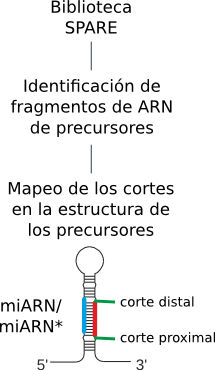
\includegraphics[width=.3\textwidth]{GR_fig1C.png}
    \caption[Esquema del procedimiento para analizar los datos de SPARE]{
        \textbf{Esquema del procedimiento para analizar los datos de SPARE.}
    }
    \label{fig:GR_fig1C}
\end{figure}

La técnica de SPARE, permite identificar los intermediarios de procesamiento de precursores de miARNs, y uniendo la información brindada por los diferentes fragmentos es posible dilucidar tanto la dirección, como el número de cortes requeridos para la biogénesis de cada miARN (Figura \ref{fig:SPARE_tecnica}).
Es decir que no sólo se puede detectar la dirección de procesamiento, sino que también la técnica permite identificar precursores que requieren más de dos cortes para liberar el miARN maduro.
Utilizamos esta técnica de SPARE para determinar el mecanismo de procesamiento cada uno de los precursores de \textit{A. thaliana}.

\begin{figure}[htbp!] 
	\centering    
	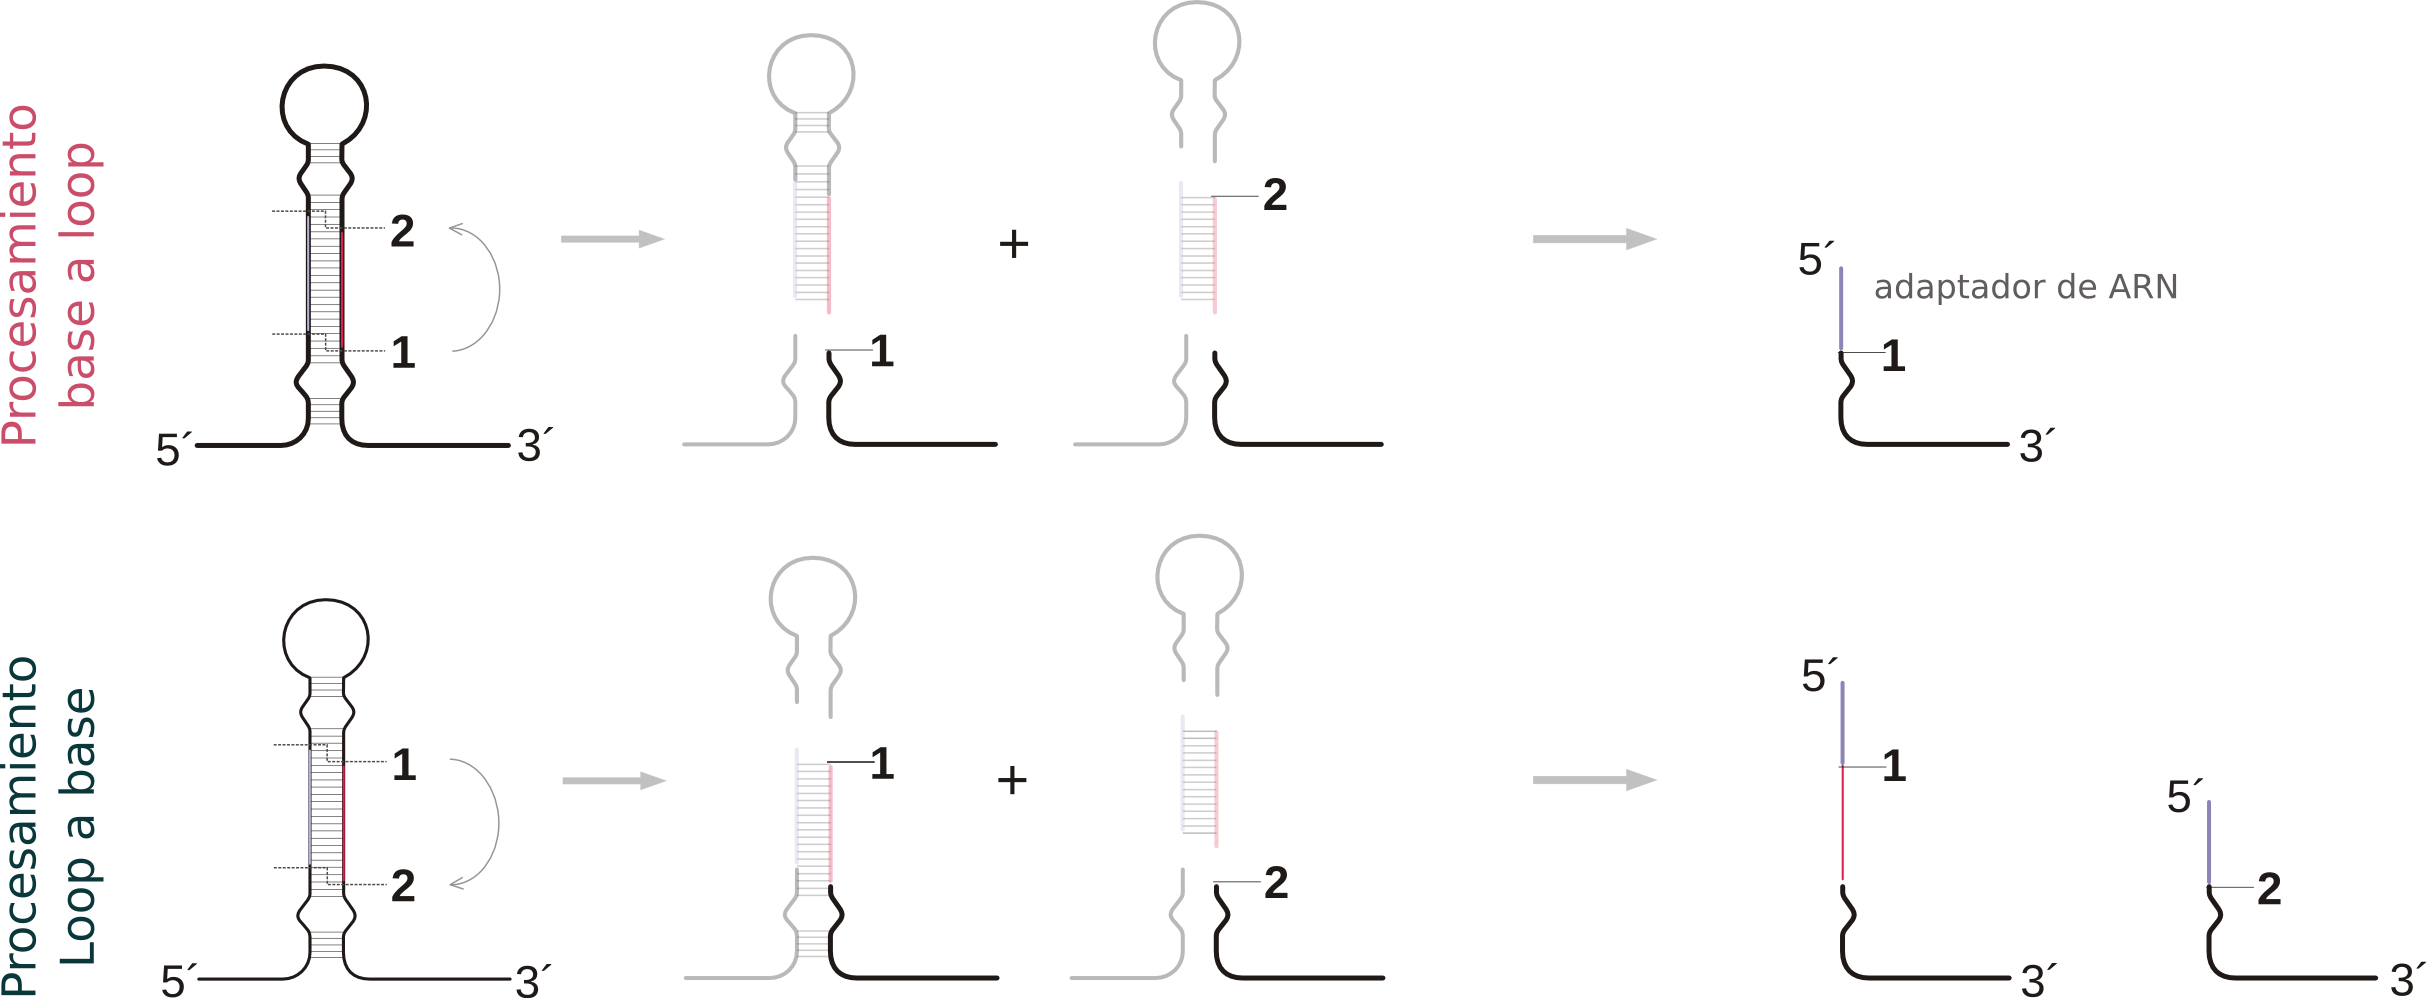
\includegraphics[width=1\textwidth]{SPARE_tecnica.png}
	\caption[Técnica de SPARE]{
        \textbf{Técnica de SPARE para diferenciar mecanismos de procesamiento de precursores.}
        Detalle donde se muestra a nivel molecular como la técnica permite diferenciar entre dos direcciones de procesamiento opuestas. 
    }
	 \label{fig:SPARE_tecnica}
\end{figure}

\subsection{Visualización de precursores que se procesan desde la base}

En el caso de los precursores que se procesan de base a loop, el único corte que puede ser detectado es el corte proximal (Figura \ref{fig:GR_fig2A}).
En la Figura se puede ver el primer corte producido por DCL1 de los precursores del miR168a, miR172a y miR395b.
Se puede observar que este corte se da $\sim$15 nt desde el loop interno por debajo del tallo inferior, y además es el único corte observado.

\begin{figure}[htbp!] 
    \centering    
    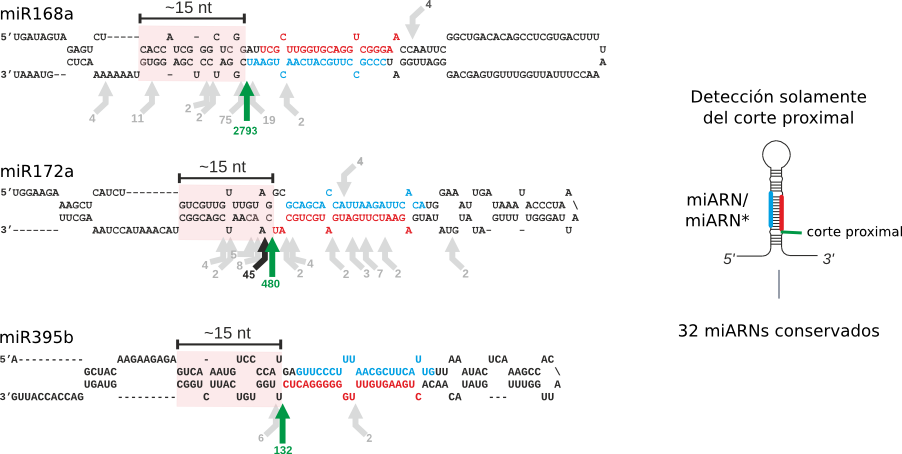
\includegraphics[width=.8\textwidth]{GR_fig2A.png}
    \caption[Identificación y caracterización de precursores de miARNs procesados de base a loop]{
    \textbf{Identificación y caracterización de precursores de miARNs procesados de base a loop.}
            Esquema donde se muestra la estructura secundaria del miR168a, miR172b y miR395b.
            Las flechas indican la posición y número de lecturas de los cortes del precursor identificado.
            Flechas en verde muestra el corte más abundante, que también coincide con al corte proximal del miARN/miARN*.
            Flechas en negro muestran otros cortes con al menos 5\% de abundancia del número total de cortes, mientras que otros cortes minoritarios se muestran con una flecha gris.
            Con rosa se resalta el stem de 15nt debajo del corte proximal.
            El miARN se indica en color rojo y el miARN* en color azul.
            La imagen de la derecha muestra el patrón de corte típico detectado en la biblioteca de SPARE para estos precursores.}
    \label{fig:GR_fig2A}
\end{figure}

\subsection{Visualización de precursores que se procesan desde el loop}

Para los precursores que se procesan de loop a base, la técnica de SPARE permite detectar tanto el corte distal como el proximal, que son los necesarios para liberar al miARN maduro (Figura \ref{fig:GR_fig4A}).
Además, en los precursores que necesitan más de dos cortes para liberar el miARN maduro, como la familia del miR319, los cuatro cortes pueden ser detectados por esta técnica.
En la figura se pueden ver los dos cortes por DCL1 de miembros de la familia del miR156 y del precursor del miR160a, que son procesados desde el loop a la base.
\begin{figure}[htbp!] 
    \centering    
    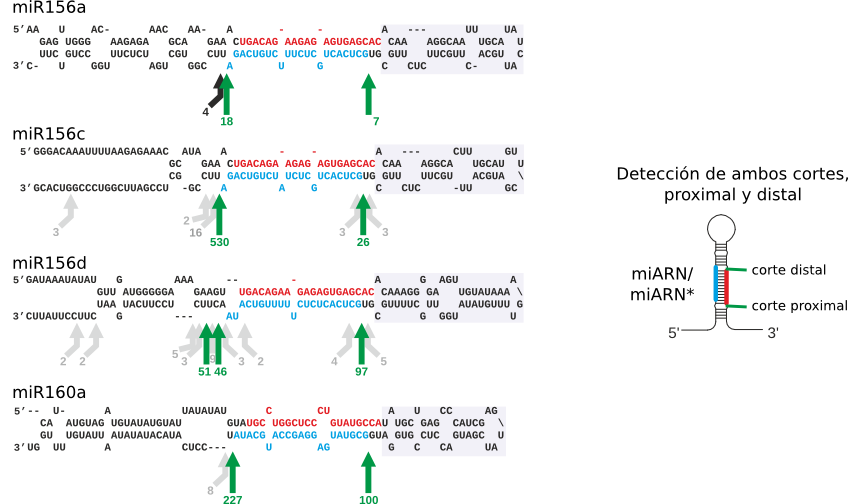
\includegraphics[width=.8\textwidth]{GR_fig4A.png}
    \caption[Identificación y caracterización de precursores de miARNs procesados de loop a base]{
    \textbf{Identificación y caracterización de precursores de miARNs procesados de loop a base.}
    Esquema donde se muestra la estructura secundaria del miR156a, miR156c, miR156d y miR160a.
    Las flechas indican la posición y número de lecturas de los cortes del precursor identificado.
    Flechas en verde muestra el corte más abundante, que también coincide con al corte proximal del miARN/miARN*.
    Flechas en negro muestran otros cortes con al menos 5\% de abundancia del número total de cortes, mientras que otros cortes minoritarios se muestran con una flecha gris.
    Con gris se resalta el stem de arriba del miR156 y miR160. El miARN se indica en color rojo y el miARN* en color azul.
    La imagen de la derecha muestra el patrón de corte típico detectado en la biblioteca de SPARE para estos precursores.
}
    \label{fig:GR_fig4A}
\end{figure}


\section{Resultados y Discusión}

\subsection{Desarrollo de herramienta para el análisis de intermediarios de procesamiento en \textit{A. thaliana}}

\subsubsection{Análisis de las bibliotecas de SPARE y diseño de la herramienta}

En una primera tanda de experimentos, Nicolás Bologna y Arnaldo Schapire realizaron bibliotecas de SPARE en Col-0 para estudiar los intermediarios de procesamiento en \textit{A. thaliana}.
De esta técnica, se obtienen una gran cantidad de datos para cada biblioteca secuenciada.
Estos datos se conocen como datos crudos y son fragmentos de secuencia que luego tienen que ser mapeados contra el genoma de datos de interés.
En este caso, el procesamiento de los datos crudos para obtener los datos finales lo realizaron en el laboratorio del Dr. Blake Meyers, que fue donde se realizaron las secuenciaciones de las bibliotecas.
Pero estos datos luego eran analizados manualmente, identificando uno por uno la posición de los cortes dentro los precursores de miARNs.

Luego, en una segunda tanda de experimentos, Belén Moro realizó nuevas bibliotecas de SPARE para precursores de \textit{A. thaliana}.
Esta nueva secuenciación se realizó debido que anteriormente no se pudieron de determinar la dirección de procesamiento de algunos precursores.
Pero además, esta nueva tanda de secuenciación, se realizó para identificar intermediarios de procesamiento en plantas mutantes en proteínas de procesamiento.
En particular, además de Col-0 se utilizaron plantas mutantes en \textit{Hyl1}, \textit{Se} y \textit{Fiery}.
Por último, en este caso, el procesamiento de los datos a partir de los datos crudos lo realizamos nosotros y se detallan en Materiales y Métodos.

Para ayudar a analizar estos datos complejos, desarrollamos una herramienta para el análisis de los datos obtenidos por la técnica de SPARE.
Esto nos permite facilitar el análisis de la identificación de los intermediarios de procesamiento en en \textit{A. thaliana}.
Primero los fragmentos son agrupados y mapeados contra las secuencias únicas de los precursores de \textit{A. thaliana} y nos quedamos con las secuencias únicas.
Esa información ya procesada es la que utilizamos en la herramienta para analizar y comparar los intermediarios de procesamiento para plantas silvestres y para las mutantes de procesamiento.

La herramienta permite seleccionar un precursor en particular de los $\sim$100 precursores que se detectaron fragmentos por la técnica de SPARE y luego se selecciona una o varias mutantes y controles que se quieren analizar.
Además la herramienta permite modificar otros parámetros como la longitud y abundancia de los fragmentos secuenciados a considerar.

\subsubsection{Precursores procesados desde la base}
Primero vemos la salida de la herramienta para el precursor del  miR165a, analizando distintas mutantes de procesamiento al mismo tiempo (Figura \ref{fig:miR165a_SPARE}).
La posición final del duplex miARN/miARN* fue considerada como la posición 0, y las posiciones positivas son bases hacia arriba del dúplex mientrás que las posiciones negativas son bases hacia abajo del dúplex.
Los fragmentos se muestran en forma porcentual tomando cada biblioteca de forma independiente y en distintos colores se representan las distintas bibliotecas.
Además se muestra una tabla con los valores absolutos de cada fragmento y con flechas verdes se marcan las posiciones con los fragmentos de mayor abundancia en promedio de todas las bibliotecas (Figura \ref{fig:miR165a_SPARE}).
 
En esta figura se muestra un precursor que es procesado con un mecanismo corto de base a loop, donde según se muestra en la Figura \ref{fig:SPARE_tecnica}, los fragmentos detectados corresponden únicamente al primer corte por DCL1 (Figura \ref{fig:miR165a_SPARE}).
Se pueden observar también cortes en las posiciones $\pm 2$ con respecto a las esperadas por actividad "sloopy" (poco rigurosa) de DCL1 \citep{pmid17989254}.
Además se observan en la posición -5, que aparecen fragmentos en todas las bibliotecas aunque en muy baja abundancia (Figura \ref{fig:miR165a_SPARE}).
Mediante esta herramienta no sólo se puede identificar los precursores procesados de base a loop o de loop a base, sino que también permite identificar a los precursores que denominamos secuenciales, que son los que requieren de más de dos cortes por DCL1 para liberar al miARN maduro.

%~ Por ejemplo, mostramos al precursor del miR169d que es procesado de forma secuencial de base a loop.
%~ En estos precursores, los sitios de cortes delestán localizados 21 nt por debajo del lado proximal del dúplex miARN/miARN* y luego DCL1 sigue cortando para procesar al precursor.
%~ En este caso se detecta un fragmento mayoritario en la posición -21, es decir 21nt por debajo del dúplex miARN/miARN* como era esperado para precursores secuenciales de base a loop \ref{fig:miR169d_SPARE}.

%~ El precursor del miR169d tiene una estructura particular donde presenta un loop terminal ramificado.
%~ Se ha estudiado este tipo de precursores, con esta estructura, donde se demostró que pueden ser procesados por DCl1 de manera bidireccional de base a loop o de loop a base, resultando en un procesamiento productivo y abortivo respectivamente \citep{pmid23934148}.
%~ Con la herramienta desarrollada por nosotros, se puede observar que este precursor particular presenta fragmentos que provienen del corte secuencial de la base al loop que corresponde a la posición -21 en el gráfico.
%~ Pero además, en la mutante de \textit{fiery} se pueden observar fragmentos que corresponden a un corte abortivo por DCL1 a partir del reconocimiento de este loop ramificado \ref{fig:miR169d_SPARE}.
%~ La herramienta permite discriminar este tipo de procesamiento en distintas mutantes de procesamiento. 

\begin{landscape}
    \begin{figure}[htbp!] 
        \centering    
        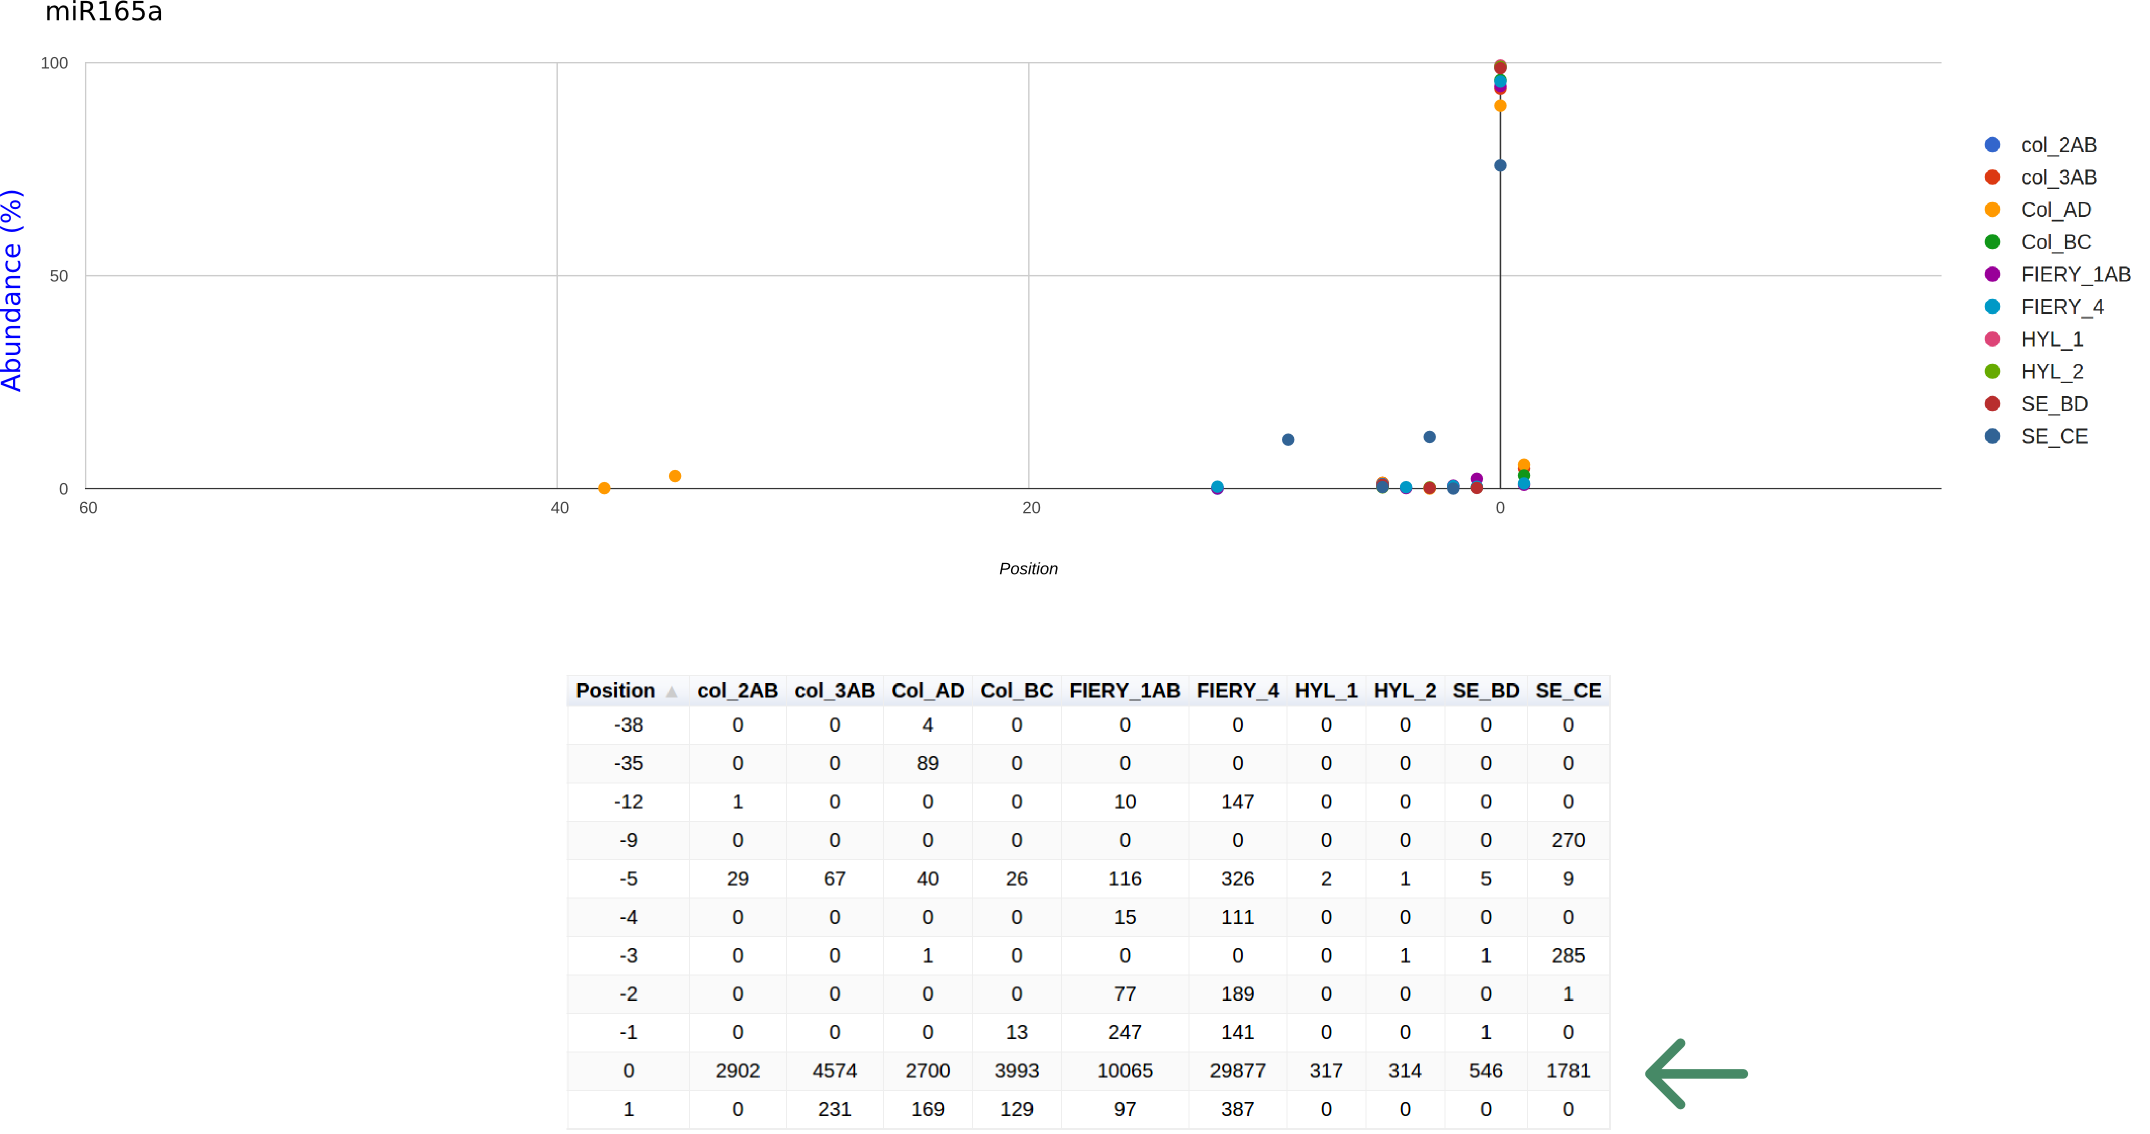
\includegraphics[width=1.4\textwidth]{miR165a_SPARE.png}
        \caption[Captura de pantalla de la herramienta de SPARE para el miR165a]{
        \textbf{Captura de pantalla de la herramienta de SPARE para el miR165a.}
        Porcentaje de fragmentos del precursor (abundancia relativa de los fragmentos en esa posición dividido la abundancia total de los fragmentos en el precursor).
        La posición final del duplex miARN/miARN* fue considerada como la posición 0.
        La tabla muestra los valores absolutos de cada fragmento.
        Las flechas verdes marcan las posiciones del precursor con los fragmentos de mayor abundancia. 
        }
         \label{fig:miR165a_SPARE}
    \end{figure}
\end{landscape}

%~ \begin{landscape}                                                                      
%~ \begin{figure}[htbp!] 
        %~ \centering    
        %~ 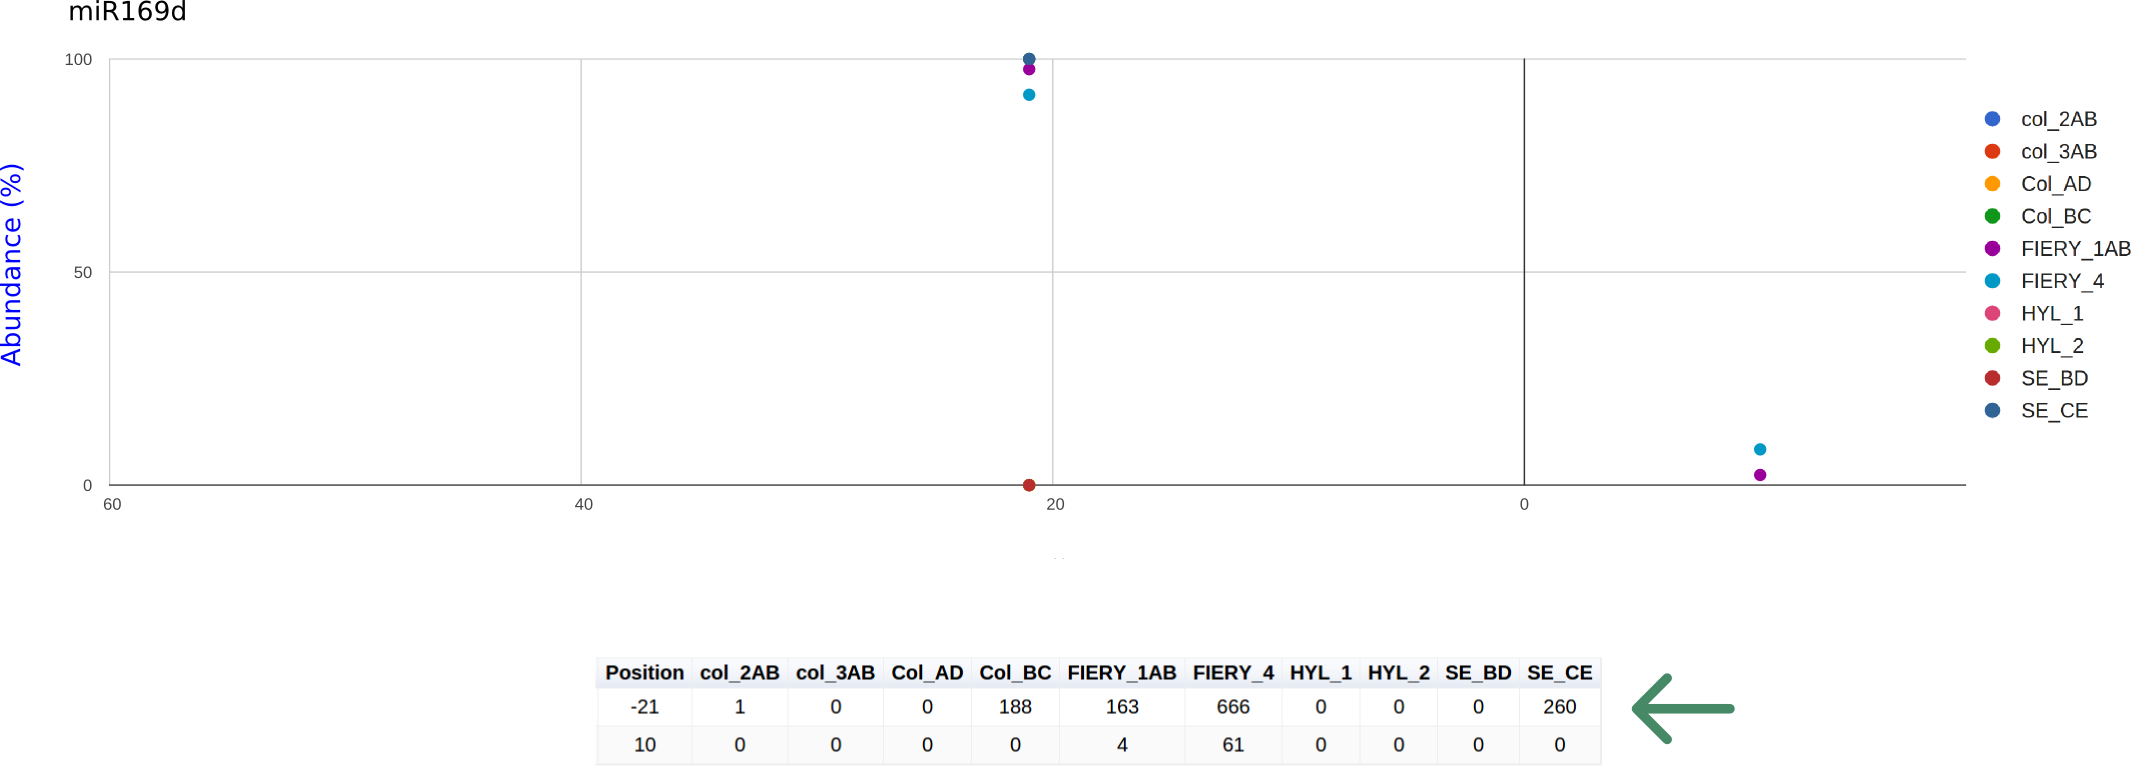
\includegraphics[width=1.4\textwidth]{miR169d_SPARE.png}
        %~ \caption[Captura de pantalla de la herramienta de SPARE para el miR169d]{
        %~ \textbf{Captura de pantalla de la herramienta de SPARE para el miR169d.}
        %~ Porcentaje de fragmentos del precursor (abundancia relativa de los fragmentos eosición dividido la abundancia total de los fragmentos en el precursor).
        %~ La posición final del duplex miARN/miARN* fue considerada como la posición 0.
        %~ La tabla muestra los valores absolutos de cada fragmento.
        %~ Las flechas verdes marcan las posiciones del precursor con los fragmentos de mayor abundancia. 
        %~ }
	 %~ \label{fig:miR169d_SPARE}
    %~ \end{figure}
%~ \end{landscape}

%~ Vemos el precursor del miR156a, donde los cortes más abundantes corresponden a las posiciones 22 y 0 (Figura \ref{fig:miR156a_SPARE}).
%~ Estos fragmentos corresponden a los cortes del precursor por DCL1, donde el primer corte se da en la parte distal del dúplex y el segundo en la parte proximal del mismo.
%~ Además se pueden observar otros fragmentos con abundancias relativas, cercanas a estas posiciones. 
%~ En algunas bibliotecas se puede observar que acumulan más el primer corte (por ejemplo la biblioteca de Col\_AD) y en otras el segundo es el más abundate (biblioteca de Fiery\_1AB) (Figura \ref{fig:SPARE_tecnica}).
%~ Esto podría ser interesante para estudiar en un futuro.
%~ Además se puede observar que en \textit{Hyl} y \textit{Serrate} hay otros fragmentos con abundancia relativa en otras posiciones que las esperadas (posición 3 y posición 14 respectivamente), sugeriendo que tal vez que los cortes podrían estar afectados en estas mutantes de procesamiento (Figura \ref{fig:SPARE_tecnica}).

\subsubsection{Precursores procesados desde el loop}

Para el caso de los precursores cortos de loop a base, los fragmentos detectados pueden ser más de uno según muestra la técnica de SPARE (Figura \ref{fig:SPARE_tecnica}).
Lo mismo sucede con los precursores de loop a base que son cortados más de dos veces por DCL1.
Para ilustrar esto, mostramos  el caso del miR159, que al igual que todos los precursores que son procesados secuenciales de loop a base, los cuatros fragmentos más abundantes corresponden a los cuatro cortes realizados por DCL1 que son requeridos para procesar este precursor (Figura \ref{fig:miR159b_SPARE}).
El primer corte se da en la posición 71, que de los cuatros cortes es el que tiene fragmentos menos abundantes, y luego DCL1 corta a 21 nucleótidos liberando otros ARN pequeños.
Luego se pueden observar los fragmentos correspondientes al tercer corte (posición 21) y cuarto corte (posición 0), que son los necesarios para liberar el miARN maduro (Figura \ref{fig:miR159b_SPARE}).
En este caso se pueden ver otros fragmentos que son productos de la degreadación del precursor, aunque nunca son tan abundantes como los fragmentos de los cortes por DCL1.
Por cuestiones de simplicidad, en la tabla solo se muestra los fragmentos con mayor abundancia en promedio de todas las bibliotecas.

%~ \begin{landscape}
    %~ \begin{figure}[htbp!] 
        %~ \centering    
        %~ 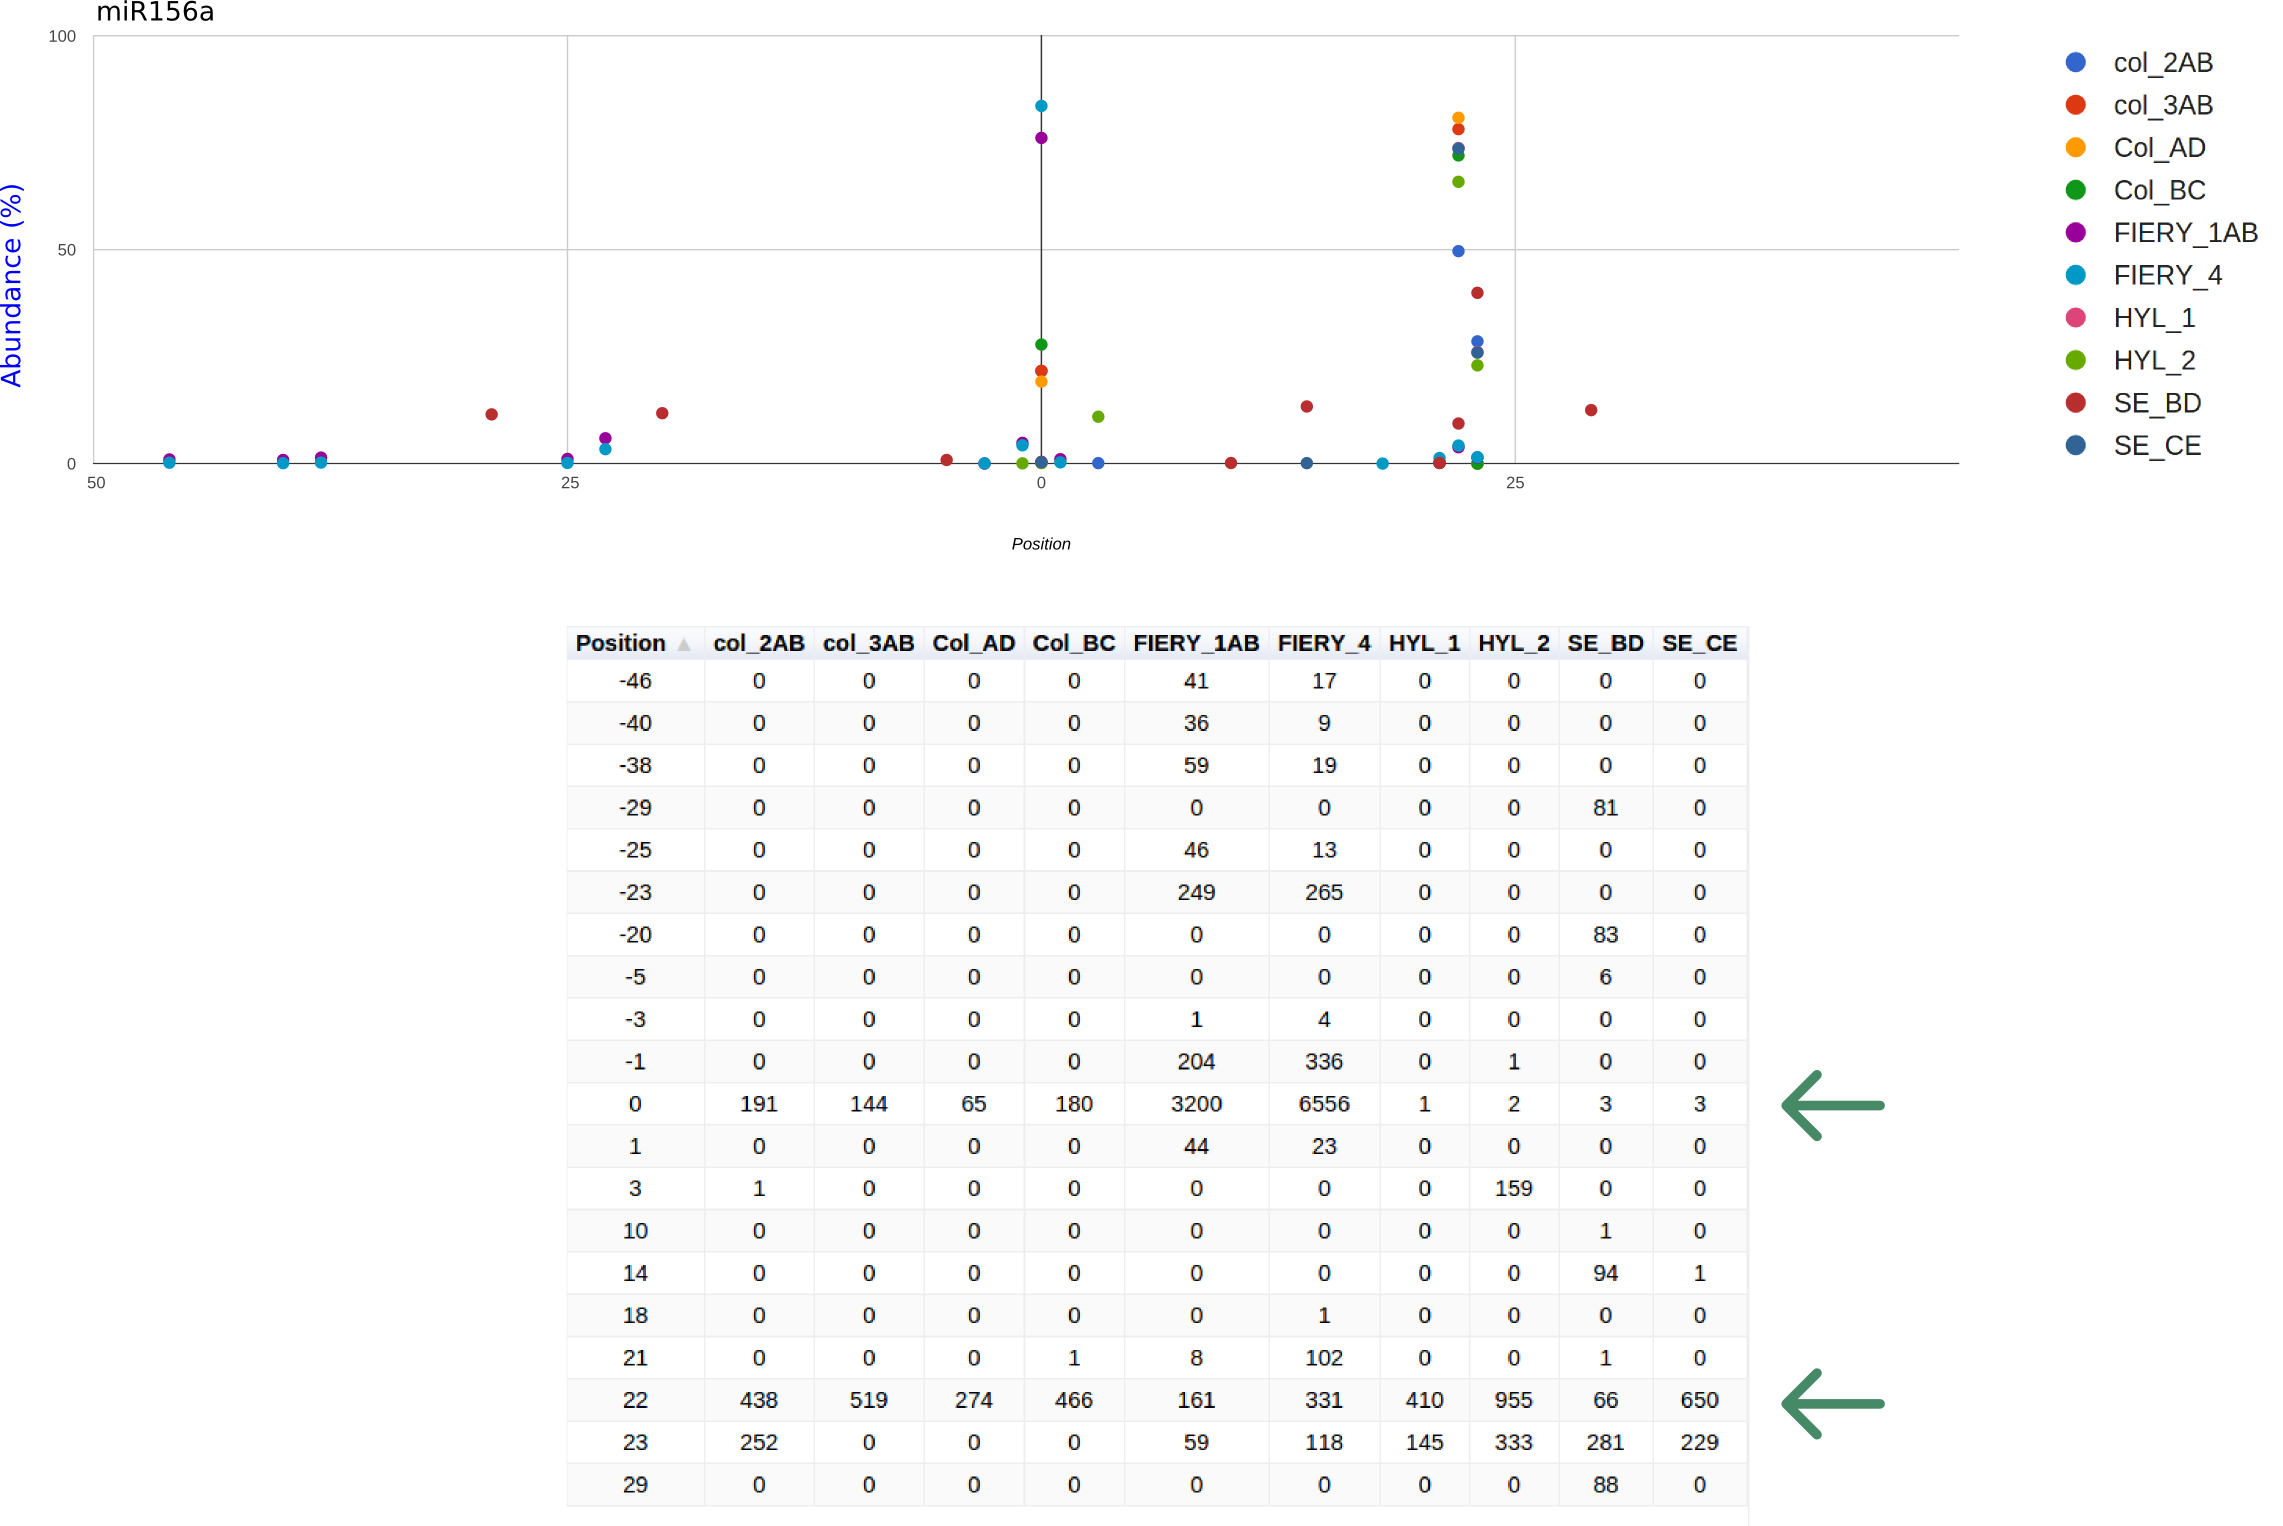
\includegraphics[width=1.4\textwidth]{miR156a_SPARE.png}
        %~ \caption[Captura de pantalla de la herramienta de SPARE para el miR156a]{
        %~ \textbf{Captura de pantalla de la herramienta de SPARE para el miR156a.}
        %~ Herramienta para analizar los datos de la técnica SPARE.
        %~ Porcentaje de fragmentos del precursor (abundancia relativa de los fragmentos en esa posición dividido la abundancia total de los fragmentos en el precursor).
        %~ La posición final del duplex miARN/miARN* fue considerada como la posición 0.
        %~ La tabla muestra los valores absolutos de cada fragmento.
        %~ Las flechas verdes marcan las posiciones del precursor con los fragmentos de mayor abundancia. 
        %~ }
         %~ \label{fig:miR156a_SPARE}
    %~ \end{figure}
%~ \end{landscape}

\begin{landscape}
    \begin{figure}[htbp!] 
        \centering    
        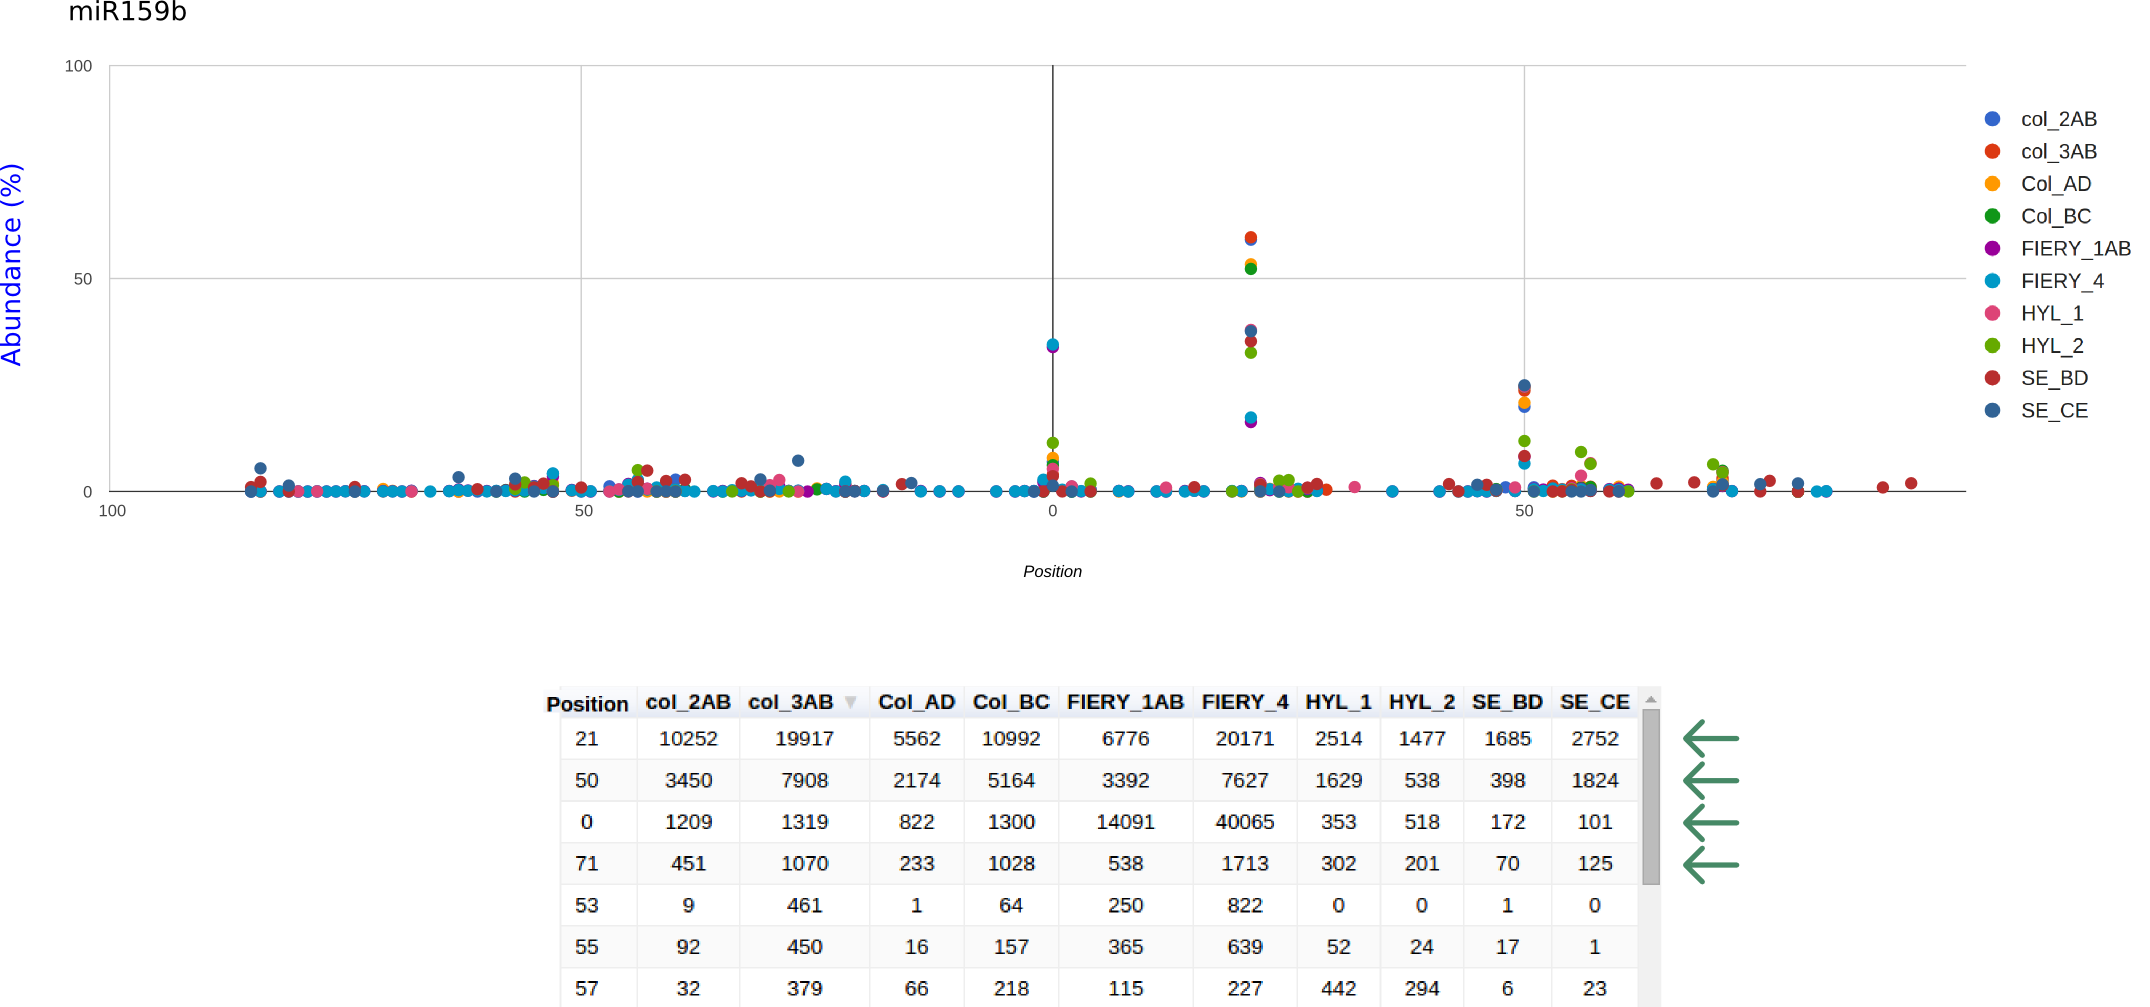
\includegraphics[width=1.4\textwidth]{miR159b_SPARE.png}
		\caption[Captura de pantalla de la herramienta de SPARE para el miR159b]{
        \textbf{Captura de pantalla de la herramienta de SPARE para el miR159b.}
        Porcentaje de fragmentos del precursor (abundancia relativa de los fragmentos en esa posición dividido la abundancia total de los fragmentos en el precursor).
        La posición final del duplex miARN/miARN* fue considerada como la posición 0.
        La tabla muestra los valores absolutos de cada fragmento.
        Por cuestiones de simplicidad, solo se muestran en la tabla los fragmentos con mayor abundancia en promedio de todas las bibliotecas.
        Las flechas verdes marcan las posiciones del precursor con los fragmentos de mayor abundancia.
        }
		\label{fig:miR159b_SPARE}
    \end{figure}
\end{landscape}


\subsection{Análisis estructural de precursores de miARNs en plantas}

Para ver si había diferencias estructurales para los precursores con diferentes mecanismos de procesamiento, determinamos la estructura secundaria de precursores detectados por SPARE de la primer secuenciación.
Obtuvimos las estructuras secundarias para cada precursor de los dos mecanismos de procesamiento, los que se procesan en dirección base a loop (Figura \ref{fig:GR_fig2C}) y los que se procesan loop a base (Figura \ref{fig:GR_fig4C}).
Definimos a una coincidencia en cada posición con un 0, mientras que "bulges" y "mismatches" los consideramos como 1.
El lado proximal del duplex miARN/miARN* fue definido como la posición +1 y analizamos desde la posición -25 a la posición +40 (Figura \ref{fig:GR_fig2C} y \ref{fig:GR_fig4C}). 

\subsubsection{Estructuras secundarias de precursores procesados desde la base}
Consideramos la estructura secundaria de precursores obtenidos a partir de la primer secuenciación, que se procesan de base a loop y todos ellos tienen un claro tallo inferior de 15 nt de largo (Figura \ref{fig:GR_fig2C}).
Además este tallo se pudo ver tanto para los precursores validados experimentalmente que se procesan de base a loop como para todos los precursores conservados (Figura \ref{fig:GR_fig2C} en violeta).
Pero pudimos observar que las bases inmediatamente debajo del duplex miARN/miARN* (posición -2 y -1) tienden a estar desapareadas (Figura \ref{fig:GR_fig2C}).
Además las posiciones -3 y -4 y las 3 últimas posiciones del stem inferior (-13,-14 y -15) están apareadas casi siempre (Figura \ref{fig:GR_fig2C}).
En general, nuestros resultados muestran que los precursores procesados en una dirección base a loop son más uniformes de lo que se pensaba previamente y que al menos algunos de los precursores no detectados como base a loop probablemente tengan otros determinantes específicos de ARN.

\begin{figure}[htbp!] 
    \centering    
    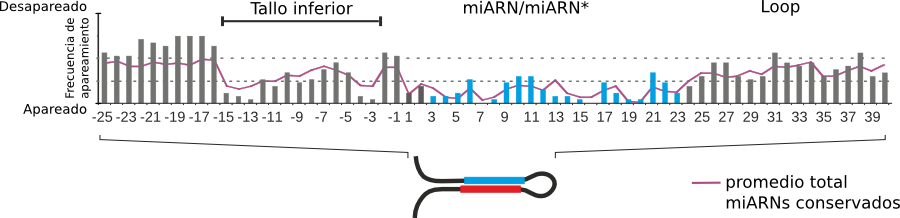
\includegraphics[width=1\textwidth]{GR_fig2C.png}
    \caption[Estructura secundaria de precursores de base a loop]{
    \textbf{Estructura secundaria de precursores detectados que se procesan en dirección base a loop.}
    Los matches en cada posición los consideramos como 0, mientras que "bulges" y "mismatches" fueron considerados como 1.
    La estructura secundaria considerando todos los miARNs conservados se indica con color violeta.
    }
    \label{fig:GR_fig2C}
\end{figure}

\subsubsection{Estructuras secundarias de precursores procesados desde el loop}
Estos precursores, que tienen un procesamiento loop a base, tienen un corte mayoritario que se puede detectar en nuestras bibliotecas.
Este corte es el esperado en la dirección de procesamiento de precursores con un mecanismo de loop a base.
Con la excepción de dos miARNs (miR396a y miR162b) estos precursores no tienen una estructura obvia debajo del duplex miARN/miARN* (Figura \ref{fig:GR_fig4C}).
Estos precursores tienen una región terminal estructurada (Figura \ref{fig:GR_fig4C}), que tiene un tamaño homogéneo de ~42nt que incluye un loop corto en contraste con la misma región en los precursores que se procesan de base a loop donde es más variable (Figura \ref{fig:GR_fig2C} y \ref{fig:GR_fig4C}). 

\begin{figure}[htbp!] 
    \centering    
    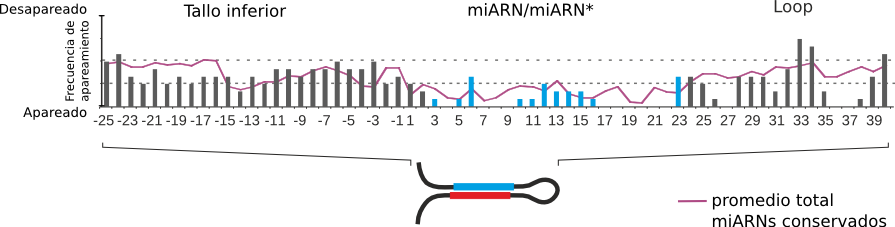
\includegraphics[width=1\textwidth]{GR_fig4C.png}
    \caption[Estructura secundaria de precursores de loop a base]{
   \textbf{ Estructura secundaria de precursores detectados que se procesan en dirección loop a base.}
    Los matches en cada posición los consideramos como 0, mientras que "bulges" y "mismatches" fueron considerados como 1.}
    \label{fig:GR_fig4C}
\end{figure}


\section{Conclusiones}

En esta segunda parte del proyecto de tesis presentamos un estrategia y realizamos un análisis sistemático para la identificación de la biogénesis de precursores de miARNs desde un punto de vista genómico.
Utilizando esta técnica encontramos que los miARNs son procesados por cuatro mecanismos, dependientes de la dirección secuencial de la maquinaria de procesamiento y del número de cortes requeridos para liberar el miARN.
La clasificación de los precursores, teniendo en cuenta los mecanismos de procesamiento, reveló determinantes estructurales específicos para cada grupo.
De esta manera pudimos encontrar la dirección de procesamiento de la mayoría de los precursores de miARNs en \textit{A. thaliana}.

Integrando los resultados que se muestran en la introducción junto a los resultados obtenidos en esta Tesis, se pudo demostrar que los precursores de miARNs en plantas se pueden agrupar por cuatro mecanismos de procesamiento con distintas características (Figura \ref{fig:mecanismos}).

\begin{itemize}
    \item En los precursores con un mecanismo \textbf{corto de base a loop}, un loop interno seguido por un tallo inferior de $\sim$15nt especifica la posición del primer corte.
        Esta estructura se encuentra en la mayoría de familias de miARNs \citep{Mateos2010,pmid20015653,pmid20015654}.
        A pesar de que el tallo puede contener bulges, la transición de un loop interno (simple hebra) al tallo inferior es bastante marcada, y tres pares de bases apareadas generalmente definen el comienzo del tallo inferior del precursor \citep{Bologna2013}.
        El segundo corte procede a una distancia fija de $\sim$21 nt desde la posición del primer corte.
    \item En los precursores con un mecanismo \textbf{secuencial de base a loop} (ej: familia del miR169), el primer corte procede como en los cortos de base a loop, pero luego son necesario dos cortes más para liberar el miARN, generando en el proceso niveles bajos de RNA pequeños adicionales \citep{Bologna2013}.
    \item En los precursores con un mecanismo \textbf{cortos de loop a base} (ej: familia del miR156 y miR160), el procesamiento es guiado por un tallo superior, y son necesarios dos cortes para liberar el miARN maduro.
        La región terminal de estos precursores tienen una largo conservado de $\sim$42 donde incluye un loop pequeño \citep{Bologna2013}.
    \item En los precursores con un mecanismo \textbf{secuencial de loop a base} (ej: familia del miR319 y miR159), cuatro cortes secuenciales por DCL1 son los encargados de procesar los precursores de miARNs.
        En general muestran un tallo largo superior, del cual otros ARNs pequeños son generados \citep{pmid19850910,Bologna2009,Bologna2013}
\end{itemize}

\begin{figure}[htbp!] 
    \centering    
    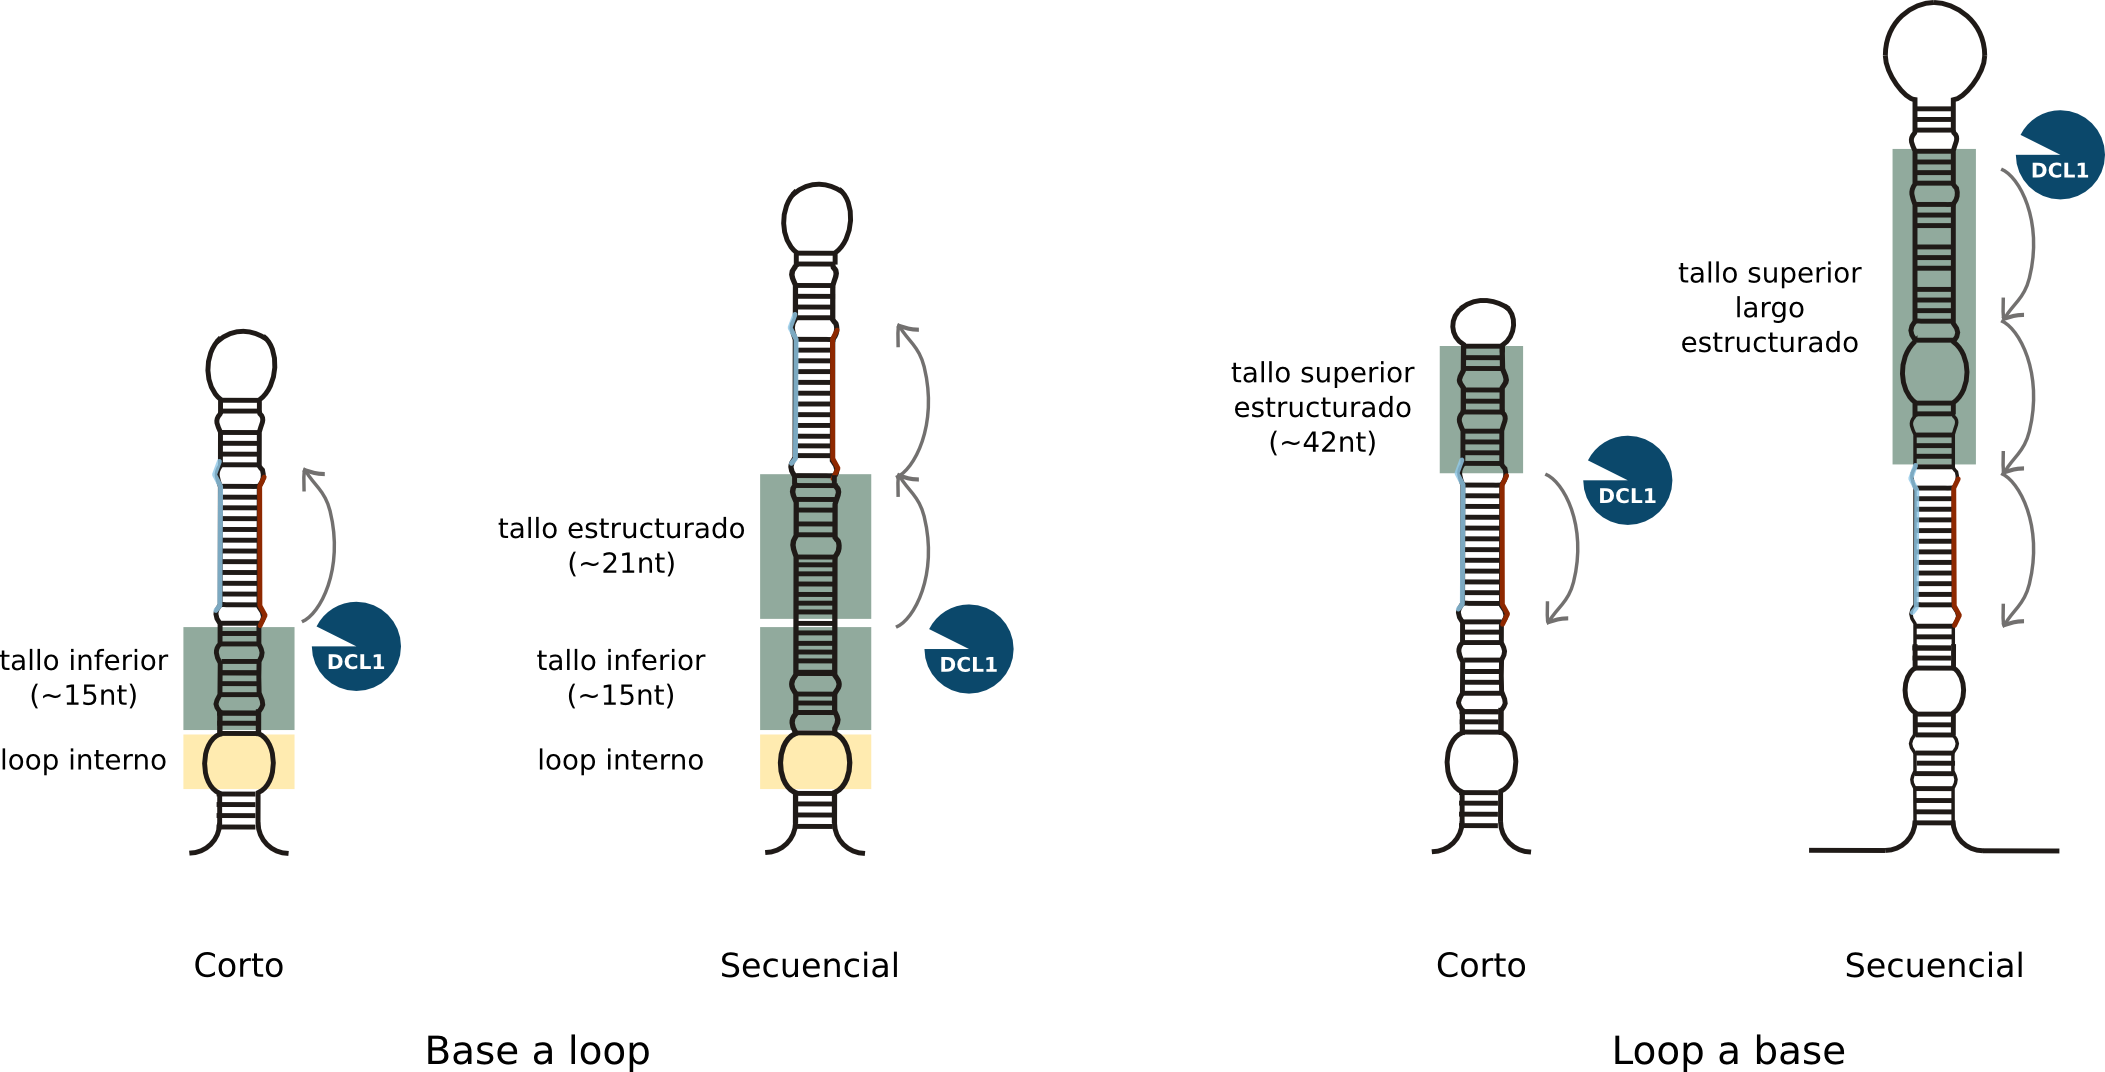
\includegraphics[width=1\textwidth]{mecanismos.png}
    \caption[Mecanismos de procesamiento]{
    \textbf{Distintos mecanismos de procesamientos de miARNs en plantas}
    A la izquierda se muestra los precursores que son procesado de base a loop.
    A la derecha se muestra los precursores que son procesado de loop a base.
    En ambos casos se muestran los precursores cortos y los secuenciales.
    Se identifica en azul el corte por DCL y con flechas la dirección de procesamiento.
        }
    \label{fig:mecanismos}
\end{figure}

Estos resultados fueron publicado en la revista Genome Research \citep{Bologna2013}.
Los resultados ofrecen una explicación para la diversidad estructural de los genes de precursores de miARN en plantas y nuevas perspectivas hacia la comprensión de la biogénesis de los ARNs pequeños \citep{Bologna2013}.

Además, utilizando estos datos de SPARE, realizamos un análisis de la estructura secundaria de precursores de \textit{A. thaliana} que tienen distintos mecanismos de procesamiento.
Y con esto, pudimos encontrar determinantes estructurales distintos para precursores que se procesados desde la base y precursores procesados desde el loop. 
